%\chapter{Final Submission}
\section{Ideas Used From Class}
\label{ideas-from-class}
\begin{itemize}
    \item Apart from Vector Space Model, we have also used SVM and gaussian naive bayes classifier to solve this classification problem.
    \item We have measured the overall F1 score of the prediction to compare the
        performance of different classification algorithms.
\end{itemize}

\section{Concepts Learned in this project}
\begin{itemize}
    \item Learnt Vector Space model which is an algebrical model for representing
        text document as a vector of index terms. This is an widely used
        technique in information retrieval.
    \item Although we studied SVM and Gaussian naive bayes classifier in our
        class, in this project we learnt how to employ them in a practical
        problem like detection of emotion from text.
    \item During the course of this project, we also became familiar with
        tf-idf (term frequency-inverse document frequency) weighting scheme.
        This is an well known technique in information retrieval which gives us
        an idea about the importance of an word to a document in a corpus.
    \item We also had a hands on experience with Weka which is a popular suite
        of machine learning algorithms. We used this tool mainly to visualize the
        training data and to test some standard classification algorithm.
\end{itemize}

\newpage
\section{Application Details}
\vspace*{-1cm}
\begin{figure}[ht!]
 \centering
 \caption{Text classifier application}
 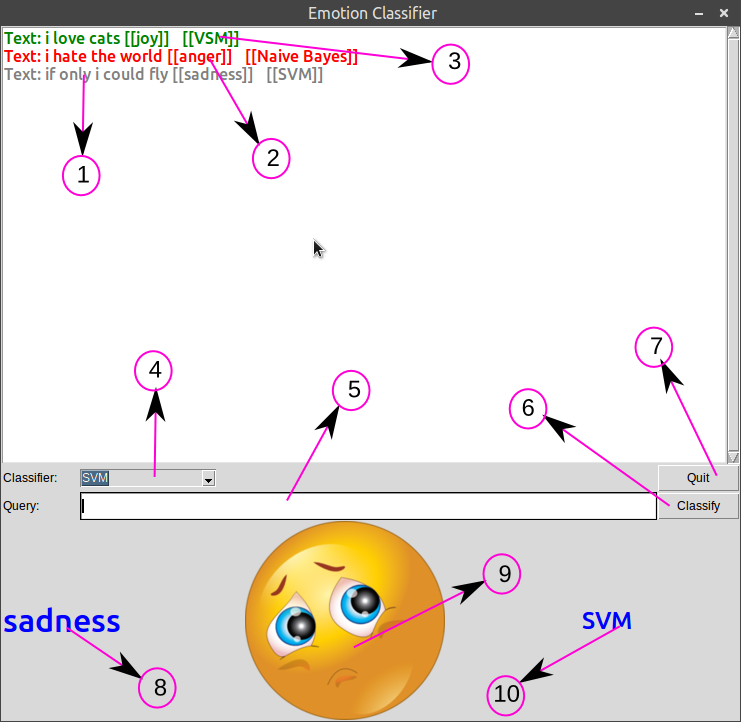
\includegraphics[width=5in,height=5in]{app} 
 \label{fig-app-shot}
\end{figure}
\vspace*{-0.5cm}
\begin{table}[ht!]
\centering
\label{tab-app-exp}
\begin{tabular}{l|c|l}
\textbf{No.} & \textbf{Element} & \textbf{Explanation}\\
\hline
1 & Text (String) & Text to be classified. \\
2 & Text (String) & The prediction made by classifier. \\
3 & Text (String) & Classifier that made the prediction. \\
4 & Combobox & Drop down showing available classifiers. \\
5 & Entry (String) & Data entered by user to query. \\
6 & Button (String) & Button to classify and print on the textbox. \\
7 & Button (String) & Button to exit the application. \\
8 & Label (String) & Large sized font - predicted emotion. \\
9 & Label (Image) & A smiley depicting the emotion. \\
10 & Label (String) & The classifying classifier. \\
\end{tabular}
\caption{Explanation of app features}
\end{table}

\section{Results}
\begin{itemize}
 \item We have throughly read the paper mentioned in \ref{paper-details}, and implemented the algorithm.
 \item There were some problems in dividing the dataset as the ISEAR dataset mentioned in \ref{dataset-details}.
 \begin{itemize}
  \item Has a total of 7 emotion classes, but for the sake of simplicity we chose to model only 3 of them.
  \item Out of the 7 classes, 6 are negative emotions (\textbf{sadness, guilt, shame, fear, anger, disgust}) and only 1 positive (\textbf{joy}).
  \item We had 2 choices now, either to divide the leftover data for 4 classes into the 2 negative ones, we've chosen (\textbf{anger,sadness}).
  \item Doing this caused a lot of misclassification, so after some research, we've currently left out 2 emotions - \textbf{guilty,fear}.
 \end{itemize}
 \item We wrote Python code to correctly implement the vector space model algorithm mentioned in \ref{subsec-high-level-alg}. We are working collaboratively and have set up a github repo to house all the data, report and code. The link is \url{https://github.com/sm88/mlproject}.
 \item Due to the above mentioned reason for less data, we are looking into some more datasets, mentioned in the paper namely, the Wordnet-Affect dataset and the Semeval dataset.
 \item The wordnet database is not available easily as we need to fill out a form, which after review will enable us to download.
 \item We have throughly cleaned the dataset, which initially had many problems. A few major ones that we solved are:
 \begin{itemize}
  \item Many sentences were of form ``No Response'', which provides no information whatsoever.
  \item There were some scattered braces and square brackets as well as some non-ascii characters, that took a while to catch.
  \item Some sentences were repeated for multiple classes.
 \end{itemize}
 \end{itemize}
 \newpage
 \subsection{Implementation related results}
 \label{subsec-impl-rel-result}
 Following are the results of applying the predictions to training data itself. Each row specifies the distribution of the samples belonging to a specific class. We trained on on 8397 sentences (documents) and then tried predicting them using our classifiers.\ref{tab-confusion-vsm}). \\

\begin{center}
	\begin{figure}[ht!]
	\label{fig-clean-dataset}	
	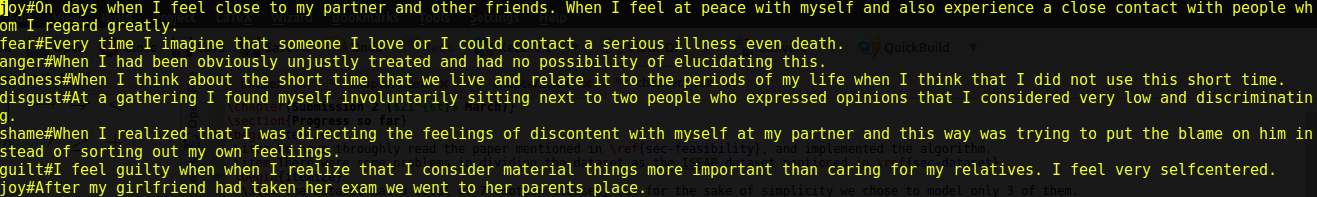
\includegraphics[width=18cm,scale=0.5]{data.png}
	\caption{Cleaned partial ISEAR dataset}
	\end{figure}
\end{center}	
\begin{table}[ht!]
  \centering
  \label{tab-confusion-vsm}
  \begin{tabular}{c|c|c|c|c}
  & \textbf{anger} & \textbf{sadness} & \textbf{joy} & \emph{Accuracy \%}\\
  \hline
  \textbf{anger} & 1745 & 469 & 201 & 72.25 \\
  \textbf{sadness} & 265 & 1832 & 258 & 77.70 \\
  \textbf{joy} & 60 & 1832 & 151 & 85.48 \\
  \end{tabular}
  \caption{Confusion matrix for training set using vsm}
\end{table}

\begin{table}[ht!]
  \centering
  \label{tab-confusion-svm}
  \begin{tabular}{c|c|c|c|c}
  & \textbf{anger} & \textbf{sadness} & \textbf{joy} & \emph{Accuracy \%}\\
  \hline
  \textbf{anger} & 2342 & 65 & 8 & 96.97 \\
  \textbf{sadness} & 70 & 2263 & 22 & 96.09 \\
  \textbf{joy} & 12 & 18 & 1424 & 97.94 \\
  \end{tabular}
  \caption{Confusion matrix for training set using svm}
\end{table}

\begin{table}[ht!]
  \centering
  \label{tab-confusion-nb}
  \begin{tabular}{c|c|c|c|c}
  & \textbf{anger} & \textbf{sadness} & \textbf{joy} & \emph{Accuracy \%}\\
  \hline
  \textbf{anger} & 1829 & 422 & 164 & 75.73 \\
  \textbf{sadness} & 5 & 1987 & 363 & 84.37 \\
  \textbf{joy} & 0 & 1 & 1453 & 99.99 \\
  \end{tabular}
  \caption{Confusion matrix for training set using nb}
\end{table}
\newpage
Following are some numbers based on unseen data for the 3 classifiers:

\begin{table}[ht!]
  \centering
  \label{tab-f1score}
  \begin{tabular}{c|c|c}
  & \textbf{f1 score} & \textbf{accuracy \%} \\
  \hline
  \textbf{vsm} & 0.436 & 44.24 \\
  \textbf{svm} & 0.403 & 40.93 \\
  \textbf{nb} & 0.459 & 47.67 \\
  \end{tabular}
  \caption{f1 score and accuracy on unseen data}
\end{table}

\section{Conclusions}
\label{sec-conclusion}
\begin{itemize}
\item We found that gaussian naive baye's outperformed the other 2 classifiers. VSM came in a close second.
\item The result is a bit expected as NB is the goto algorithm for text classification. Since we are using continuous valued attributes (tf-idf weights) GNB was an obvious choice.
\item In our opinion SVM performed poorly because of the nature of the data. First of all it was sparse and secondly there was quite a bit of overlap in the data.
\item If a word is not present in the lexicon, the prediction accuracy suffers highly.
\item In VSM we tried other measures of similarity but again due to the nature of data reverted back to cosine similarity, as it is considered best for sparse data. Other measures like euclidian distance, rbf-kernel are also used but cosine similarity outperforms them over sparse data.
\end{itemize}

\newpage
\section{Future Work}
\label{sec-plan-for-sem}
\begin{enumerate}
 \item We can try and find more patterns in the dataset like the one shown in the paper. There they've created new words from negative verbs. For example, the input sentence ``I don't love you.'' is transformed to ``I do not love you.'' which is again transformed to ``I do NOTlove you''. Here we see that finally a new word \emph{NOTlove} has been created. Authors claim this helps increase accuracy.
 \item We can find set differences between various classes on basis of words (words unique to each emotion class), and remove them from stop words list for accurate predictions.
 \item We can implement naive baye's classifier using bi-gram, tri-gram etc approaches.
 \item We can also do sentiment analysis of our dataset where we will just check the accuracy of negative and positive emotions(binary classification).
 \item We can apply some unsupervised learning technique in this problem which will be useful when availability of large annotated dataset is very low.
\end{enumerate}
\section{Pointers to literature}
\begin{itemize}
 \item The wordnet-affect dataset can be accessed from \url{http://wndomains.fbk.eu/wnaffect.html} although we need to fill out some forms before we are granted a download link.
 \item The Semeval task 14, is a medical dataset available at \url{http://alt.qcri.org/semeval2015/task14/index.php?id=data-and-tools}.
 \item Multinomial naive baye's using \textbf{tf-idf} technique can be found at \url{http://sebastianraschka.com/Articles/2014_naive_bayes_1.html}.
 \item As mentioned in section \ref{sec-plan-for-sem}, SVM could be useful for classification. The paper at \url{http://www.cs.cornell.edu/people/tj/publications/joachims_98a.pdf} presents a good use case.
 \item For naive baye's we could also add the chi-squared test for confidence computation. Some details are outlined in \url{http://www.dis.uniroma1.it/~leon/didattica/webir/IR11.pdf}.
 \item Code listing is attached and is publicly available at \url{https://github.com/sm88/mlproject}.
\end{itemize}

